\documentclass[aspectratio=169, 14pt]{beamer}
\usepackage[utf8]{inputenc}
\usepackage{xeCJK}
\usepackage{graphicx}
\usepackage{transparent}
\usepackage[ruled, lined, linesnumbered, commentsnumbered]{algorithm2e}
\usepackage{pgfplots}
\usepackage{tikz}
\usetikzlibrary{matrix,backgrounds}
\usetikzlibrary{arrows}
\usetikzlibrary {arrows.meta}
\usetikzlibrary{calc,shadows.blur,fit,positioning}
\usetikzlibrary{chains}
\usepackage{minted}
\usepackage{fontawesome5}
\usepackage{booktabs}
\usepackage{caption}
\usepackage{hyperref}
\hypersetup{
    colorlinks=true,
    linkcolor=blue,
    filecolor=magenta,      
    urlcolor=cyan,
    }
\urlstyle{same}
\usetheme{metropolis}
\metroset{block=fill}
\usecolortheme{default}
\definecolor{darkmidnightblue}{rgb}{0.0, 0.2, 0.4}
\definecolor{LightGray}{gray}{0.9}


%------------------------------------------------------------
%This block of code defines the information to appear in the
%Title page
\title[Database Principles and Applications] %optional
{数据库原理与应用}

\subtitle{ER模型}

\author[CHEN Zhongpu] % (optional)
{CHEN Zhongpu}

\institute[] % (optional)
{
  School of Computing and Artificial Intelligence \\
  \href{mailto:zpchen@swufe.edu.cn}{zpchen@swufe.edu.cn}
}

\date[] % (optional)
{SWUFE, Fall 2022}

%End of title page configuration block
%------------------------------------------------------------


%------------------------------------------------------------
%The next block of commands puts the table of contents at the 
%beginning of each section and highlights the current section:

% \AtBeginSection[]
% {
%   \begin{frame}
%     \frametitle{Table of Contents}
%     \tableofcontents[currentsection]
%   \end{frame}
% }
%------------------------------------------------------------


\begin{document}

%The next statement creates the title page.
\frame{\titlepage}

%---------------------------------------------------------
%This block of code is for the table of contents after
%the title page
% \begin{frame}
% \frametitle{Table of Contents}
% \tableofcontents
% \end{frame}
%--------------------------------------------------------
\begin{frame}
    \frametitle{复习}
    \begin{center}
        \LARGE {\faIcon{database}}
    \end{center}
    \begin{enumerate}
        \item 如何使用数据库
        \item 如何设计数据库
        \item 如何实现数据库
    \end{enumerate}

\end{frame}

{
    % \usebackgroundtemplate{\transparent{0.3}{\begin{picture}
    %     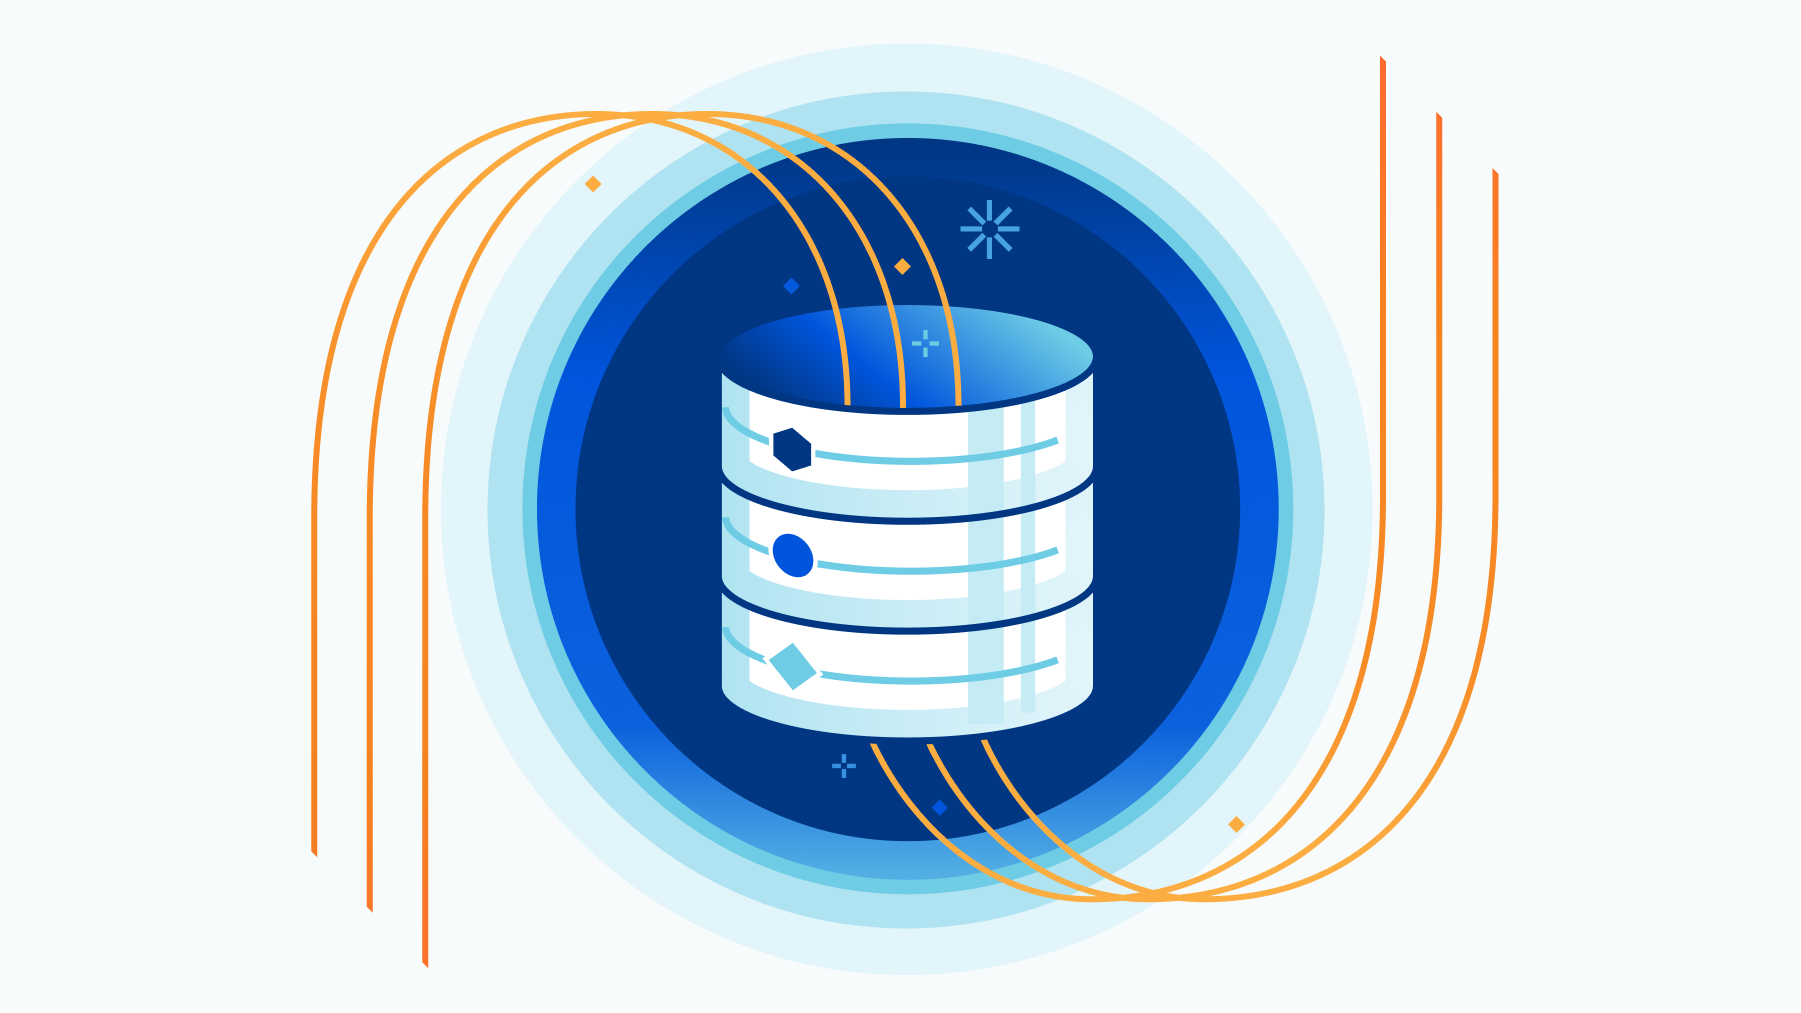
\includegraphics[height=0.7\paperheight]{cover}
    % \end{picture}    
    % }}
\usebackgroundtemplate{
  \tikz[overlay,remember picture] 
  \node[opacity=0.3, at=(current page.south east),anchor=south east, yshift=2cm,xshift=4cm] {
    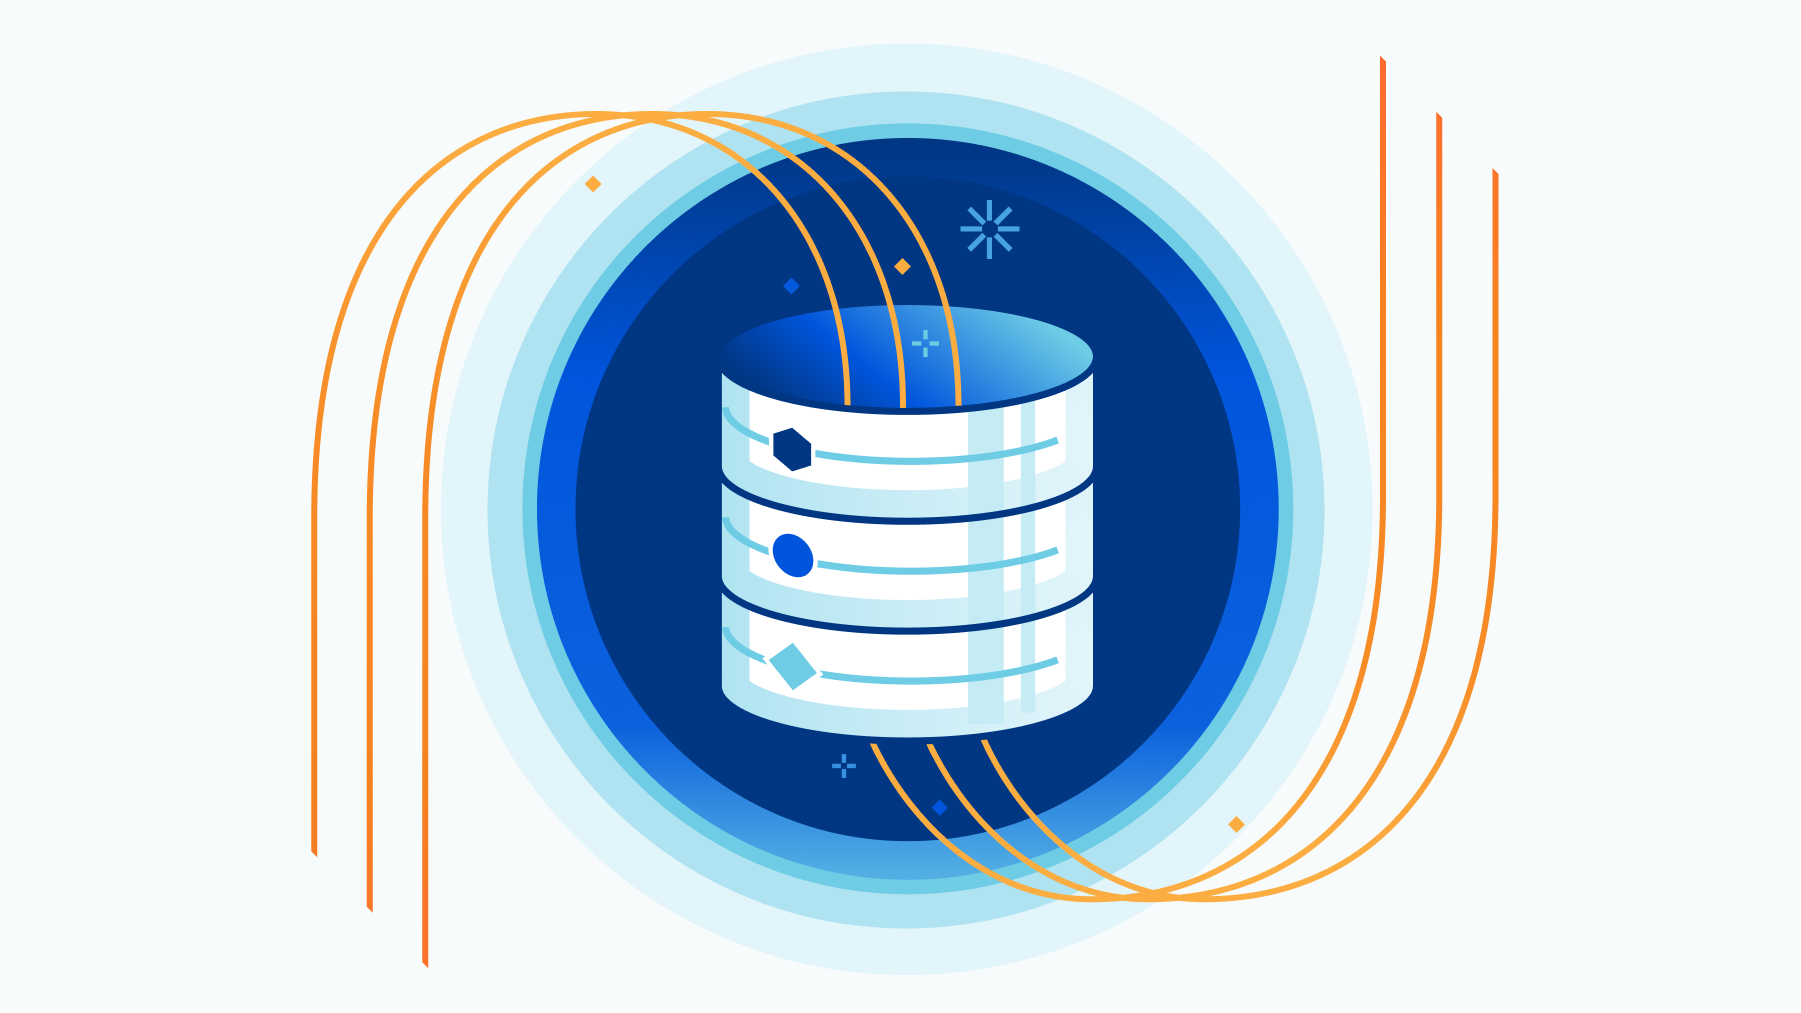
\includegraphics[height=0.6\paperheight]{cover}};
}
    \begin{frame}
        \section{\textcolor{darkmidnightblue}{1. 数据库设计概览}}
        如何将「需求」变成最终设计?
    \end{frame}
}

\begin{frame}
    \frametitle{1.1 设计阶段}
    对小型应用,一个数据库的设计者一般可以直接决定要构建的关系、关系的属性及其上的约束。

    但现实中的应该一般非常复杂,通常没有一个人能够理解应用的全部需求,所以为了沟通需求,应该将用户的需求\alert{分阶段}地用某种\alert{高级别}的方式表示出来,最后再将需求转化为\alert{较低级别}的设计。
\end{frame}

\begin{frame}[fragile]
    \begin{tikzpicture}[>=stealth,
        node distance = 3mm and 3mm,
          start chain = A going below right,
    every node/.style = {draw, text width=24mm, minimum height=12mm, align=center,
                         inner sep=1mm, fill=white, drop shadow={fill=black},  on chain=A},
                            ]
    \node (nreq) {需求分析}; % A-1
    \node {概念设计};
    \node {逻辑设计};
    \node {物理设计};
    %
    \foreach \i [count=\j] in {2,...,4}
    {
    %   \draw[->, thick] (A-\i) -| (A-\j);
      \draw[->, thick] (A-\j) -| (A-\i);
    }
    \end{tikzpicture}

    \begin{tikzpicture}
        \node[fill=blue!30,blur shadow={shadow xshift=-0.5ex},
        text width=16em,anchor=south west,rounded corners]
        {参考课本 p. 208:图7.2。};
    \end{tikzpicture}

\end{frame}

\begin{frame}[fragile]
    \frametitle{1.2 关于需求}
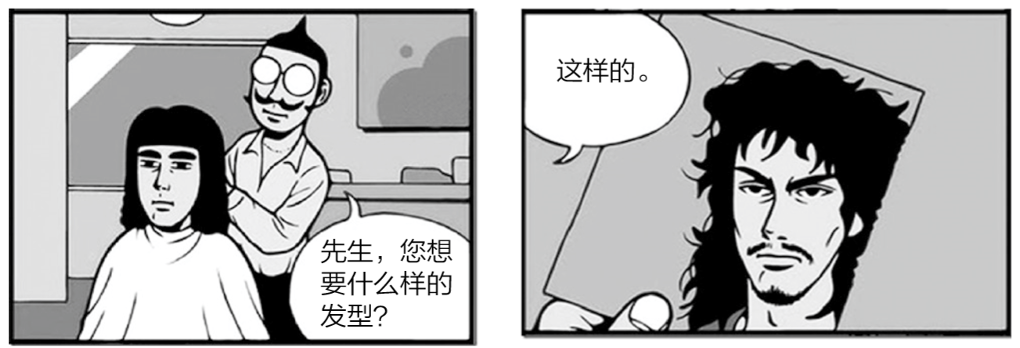
\includegraphics[width=.8\textwidth]{week10/hair1}

\pause
\begin{columns}
    \column{.4\textwidth}
    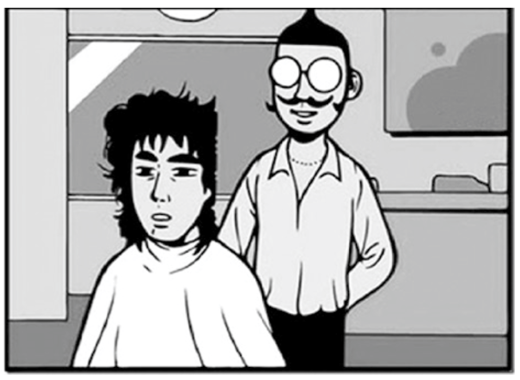
\includegraphics[width=.9\textwidth]{week10/hair2}
    \column{.6\textwidth}
    \begin{tikzpicture}
        \node[fill=yellow,blur shadow={shadow xshift=-0.5ex},
        text width=16em,anchor=south west,rounded corners]
        {理解用户的需求并不简单,并且可能用户也不知道自己的需求。};
    \end{tikzpicture}
\end{columns}

\end{frame}

\begin{frame}
    \frametitle{思考}

\begin{columns}
    \column{.5\textwidth}
    数据库设计并运行后,修改 \rule{1cm}{0.15mm} 相对比较简单。

\begin{itemize}
    \item 逻辑模式
    \item 物理模式
\end{itemize}
    \column{.5\textwidth}
    \begin{tikzpicture}[
        node distance=2cm,
        title/.style={font=\color{black!50}\ttfamily, fill=orange!30,},
        typetag/.style={rectangle, draw=black!50, font=\ttfamily, anchor=west}
      ]
        \node (decomp) [title] { \normalsize 视图层 (view level)};
      
        \node (di) [below=of decomp.west, typetag, yshift=0.5cm] { view 1 };
        \node (dr) [right=of di.west, typetag] { view 2 };
        \node (dots) [right=of dr.west] {...};
        \node (dnc) [right=of dots.west, typetag, xshift=-1cm] { view n };
      
        \node [draw=black!50,  fit={(decomp) (di) (dr) (dots) (dnc)}] (view){};
    
        \node[draw=black!50, below=of view, yshift=1cm,title](logical){逻辑层 (logical level)};
    
        \node[draw=black!50, below=of logical, yshift=1cm,title](physical){物理层 (physical level)}; 
    
        \draw[-, thick] (view) -- (logical);
        \draw[-, thick] (logical) -- (physical);
    
      \end{tikzpicture}
\end{columns}

\end{frame}


\begin{frame}
    \section{\textcolor{darkmidnightblue}{2. E-R模型}}
    实体(entity)-联系(relationship)模式在将现实世界的需求映射到概念模式上非常有用。
\end{frame}

\begin{frame}
    \frametitle{历史}
\begin{columns}
    \column{.3\textwidth}
    \begin{figure}
        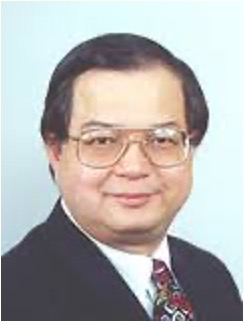
\includegraphics[width=\textwidth]{week10/chen}
        \caption*{Peter Pin-Shan Chen
        \\ 陳品山}
    \end{figure}
    \column{.69\textwidth}
    In software engineering, an ER model is commonly formed to represent things a business needs to remember in order to perform business processes. Consequently, the ER model becomes an abstract data model, that defines a data or information structure which can be implemented in a database, typically a relational database. 
\end{columns}

\end{frame}

\begin{frame}
    \frametitle{2.1 实体与实体集}
与关系模式类似,实体(entity)通过一组属性表示。

\begin{exampleblock}{实体与实体集}
实体是现实世界中可区别所有其他对象的一个“事物”或“对象”。实体集(entity set)是相同类型的一个实体集合。    
\end{exampleblock}

\end{frame}

\end{document}